\section{Predictions for MICADO's point source sensitivity}
\label{sec:micado}

MICADO will offer diffraction-limited imaging with a PSF width of about 7 and 12 milli-arcseconds in the J and Ks filters respectively.
This will allow stars in densely populated regions such as the centres of globular clusters to be easily resolved (an example is shown in Fig.~\ref{fig:stellar_field_comp}).
Indeed the majority of the primary science cases for MICADO revolve around accurately resolving points sources.
Thus it is imperative to know the sensitivity limits of the imaging mode well in advance of MICADO going on-sky.
Here we present the results of a series of SimCADO simulations aimed at determining the observational limits for MICADO.
The model of the optical train used for these simulations was the default MICADO wide-field imaging mode.
The method for measuring the signal-to-noise ratio was identical to the method used for the HAWK-I verification run described in Sect.~\ref{sec:hawki}, except the minimum integration time was extended to 2.6\,seconds.
This reflects the read-out time of the HAWAII-4RG detectors.
Also the grid of stars used for the test observations included only stars with (Vega) magnitudes between 16 and 32 as the extended diffraction spikes from stars brighter than 16th magnitude extended into the background annuli used for photometry of the neighbouring stars.
% The extent to which such PSF artefacts influence the accuracy of both the photometry as well as the completeness of observed stellar populations is indeed an important question and will be addressed in a companion paper. For this study, however, we simply removed the stars whose PSF artefacts contaminated their neighbours' apertures.

The PSFs for these simulations were produced by the SCAO working group for the MICADO consortium (F. Vidal, private communication) specifically for inclusion in the SimCADO package.
They were generated using the current state-of-the-art adaptive optics simulations and describe the residual PSF after the AO loop has been closed.
The simulations were run for a 14.7\m guide star that is $5\arcsec$ off-axis.
The targets were observed at the zenith.
The Strehl ratios of the PSFs were 0.29, 0.51 and 0.68 for the J, H and Ks band respectively.
It should be noted that such Strehl ratios are only to be expected within a region $\sim5\arcsec$ around the SCAO guide star\footnote{Readers interested in simulating SCAO observations at different positions inside the MICADO field of view are directed to see the the python package AnisoCADO: \url{https://anisocado.readthedocs.io/}. AnisoCADO produces SCAO PSFs for any combination of observation conditions and NGS positions for the ELT optical system.}.
For regions further afield, the SCAO strehl ratio drops quickly.
Additionally MCAO corrections will most likely never attain such high Strehl ratios, simply due to physical constraints of an MCAO system.
Hence these estimates are to be taken as optimistic detection limits for point source based science cases.


\subsection{Point source sensitivity vs. exposure time}
\label{subsec:MICADO_sensitivities}

\begin{figure*}

    \centering
    % 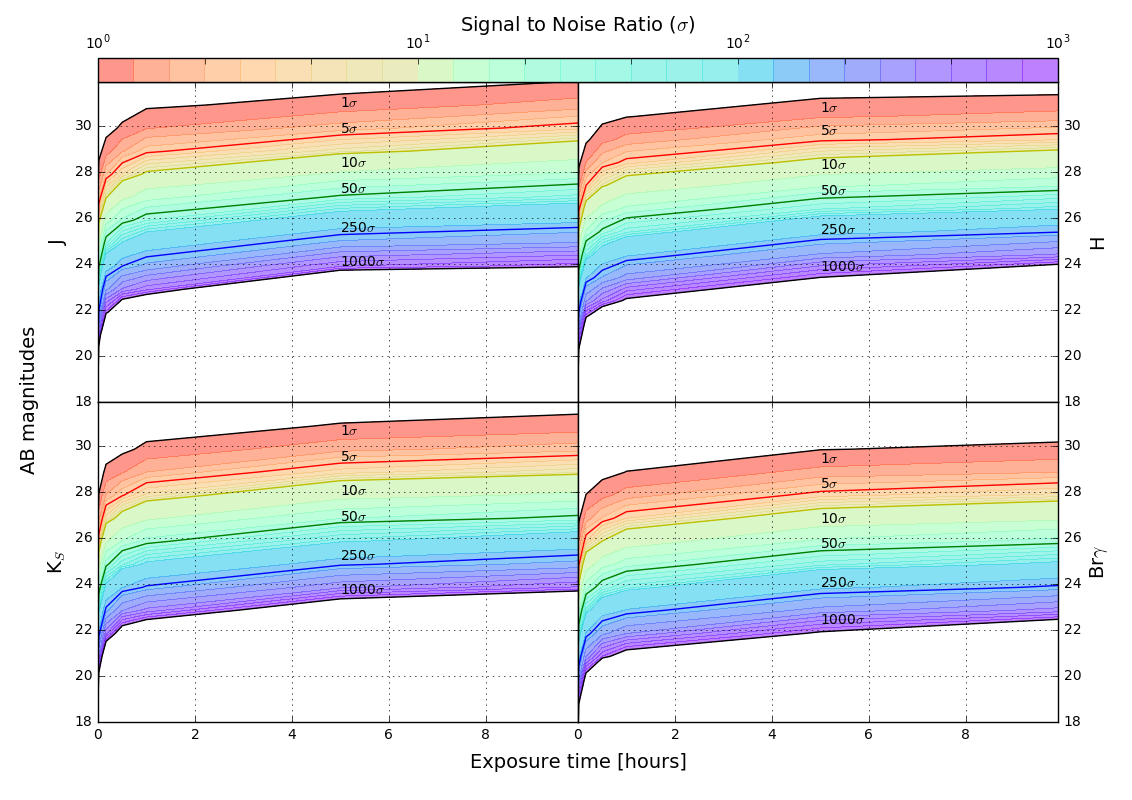
\includegraphics[width=\textwidth]{images/MICADO_SNR_Rainbow_JHKBrG_ab}
    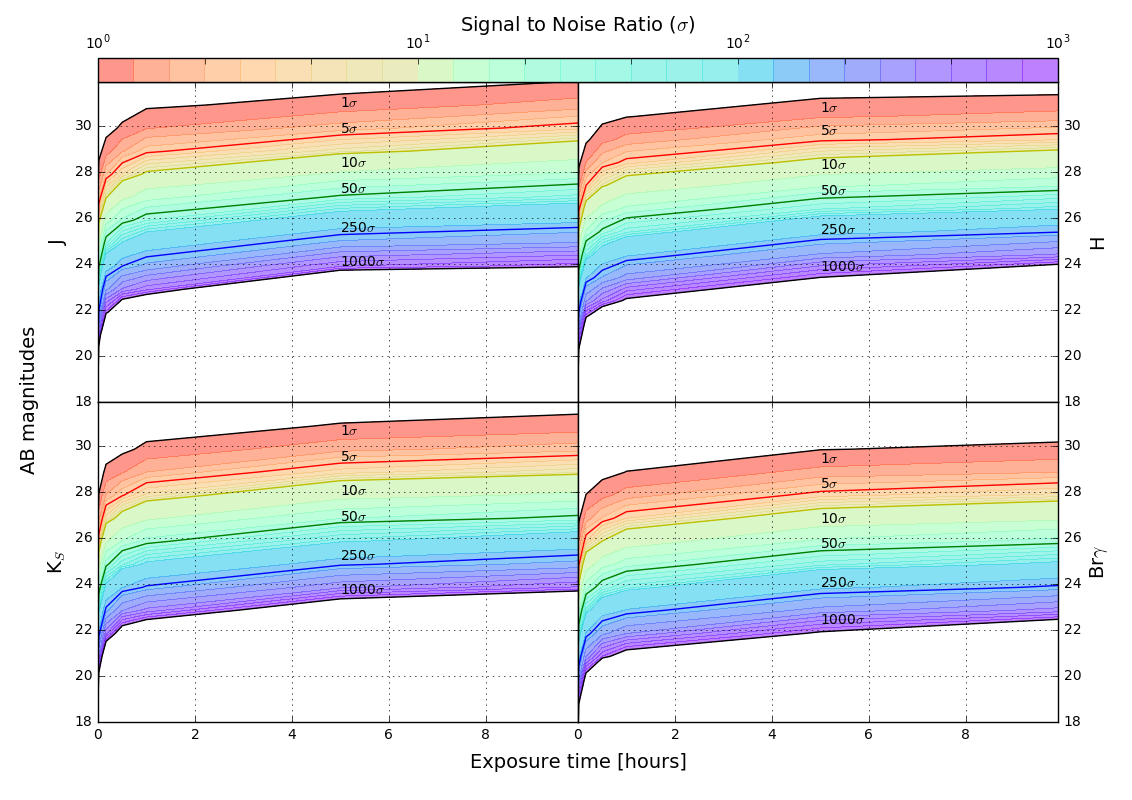
\includegraphics[width=\textwidth]{images/MICADO_SNR_Rainbow_JHKBrG_ab}

    \caption{Limiting magnitude plots for the wide field (4\,mas/pixel) imaging mode of MICADO at the ELT in Vega magnitudes.
    Signal-to-noise ratios above $5\sigma$ are sufficient for photometry.
    High precision astrometry requires stronger detections $\sim 250\sigma$.
    It should be noted that these magnitudes apply to the current design of MICADO and the ELT.
    At the time of publication MICADO is still in its design phase.
    As such we expect small changes in these values as the MICADO design matures.}
    
    \label{fig:point_source_sensitivities}
    
\end{figure*}


% 5hr  ETC JHK 28.7  27.9  27.5   M1 Area is 10% larger, but we used SCAO with 50% SR. They used wider filters, but higher BG
% 2.6s ETC JHK 23.6  23.1  22.5
% Sat  ETC JHK 15.8  15.6  14.9   M1 Area is 10% larger, pixels 5mas, SNR~750 After normalising they fit


% \begin{table*}

%     \centering
%     \caption{Specific point-source sensitivities for the NIR broadband filters J, H and Ks and the narrow band filter \brgamma. $5\sigma$ and $10\sigma$ are generally accepted detection limits for photometric measurements, while for accurate astrometry signal-to-noise ratios above $250\sigma$ are required. The errors on these magnitudes are $\pm 0.1$\m. It should be noted that these magnitudes apply to the current design of MICADO and the ELT. At the time of publication MICADO is still in its design phase. As such we expect small changes in these values as the MICADO design matures.}
%     \label{tbl:micado_point_source_sensitivities}

%     \begin{tabular}{ l r | r r r r r r r }
%         \hline\hline
% Filter          & SNR       & 2.6 sec & 10 sec    & 1 min     & 10 min    & 1 hr      &  5 hrs    & 10 hrs   \\
%         \hline
%                 & 5\sig     & 23.4\m  &   24.4\m  &   25.6\m  &   26.7\m  &   27.8\m  &   28.7\m  &   29.0\m   \\
%     J           & 10\sig    & 22.6\m  &   23.6\m  &   24.8\m  &   26.0\m  &   27.0\m  &   27.9\m  &   28.2\m   \\
%                 & 250\sig   & 18.7\m  &   19.9\m  &   21.1\m  &   22.4\m  &   23.4\m  &   24.2\m  &   24.6\m   \\
%         \hline
%                 & 5\sig     & 23.0\m  &   23.8\m  &   24.8\m  &   26.0\m  &   27.0\m  &   27.9\m  &   28.3\m   \\
%     H           & 10\sig    & 22.2\m  &   23.0\m  &   24.0\m  &   25.3\m  &   26.2\m  &   27.1\m  &   27.5\m   \\
%                 & 250\sig   & 18.6\m  &   19.4\m  &   20.4\m  &   21.7\m  &   22.7\m  &   23.5\m  &   23.9\m   \\ 
%         \hline
%                 & 5\sig     & 22.4\m  &   23.1\m  &   24.1\m  &   25.6\m  &   26.4\m  &   27.3\m  &   27.7\m   \\
%     Ks          &  10\sig   & 21.6\m  &   22.4\m  &   23.4\m  &   24.8\m  &   25.6\m  &   26.5\m  &   26.9\m   \\
%                 &  250\sig  & 18.0\m  &   18.9\m  &   19.8\m  &   21.0\m  &   22.1\m  &   22.9\m  &   23.3\m   \\
%         \hline
%                 & 5\sig     & 20.6\m  &   21.8\m  &   22.9\m  &   24.1\m  &   25.2\m  &   26.0\m  &   26.3\m   \\
%     \brgamma    & 10\sig    & 19.8\m  &   21.0\m  &   22.1\m  &   23.4\m  &   24.4\m  &   25.2\m  &   25.6\m   \\
%                 & 250\sig   & 16.0\m  &   17.1\m  &   18.4\m  &   19.8\m  &   20.8\m  &   21.7\m  &   22.1\m   \\
%         \hline
        

%     \end{tabular}
     
        
% \end{table*}

\begin{table}

    \centering
    \caption{Specific point-source sensitivities for the NIR broadband filters J, H and Ks and the narrow band filter \brgamma.
    The $5\sigma$ detection limits of a 5 hour exposure are given below in AB and Vega magnitudes and are valid for strehl ratios of 29\%, 51\%, and 68\% in the J, H and Ks filters.
    The errors on these magnitudes are $\pm 0.1$\m.}
    \label{tbl:micado_point_source_sensitivities}

    \begin{tabular}{ l | c c c c }
        \hline\hline
Filter          & J         & H        & Ks         & Br $\gamma$   \\
        \hline                
    AB          & 29.6\m    & 29.3\m   & 29.1\m     & 27.0\m        \\
        \hline                
    Vega        & 28.7\m    & 27.9\m   & 27.3\m     & 26.0\m        \\
        \hline                
    \end{tabular}

\end{table}


For studies of stellar populations, the detection limit is often set to $5\sigma$.
% , where $\sigma$ is the level of total background noise inside an aperture set around a star. 
Table~\ref{tbl:micado_point_source_sensitivities} lists MICADO's limiting magnitudes for the photometric case in the AB and Vega magnitude systems.
Fig. \ref{fig:point_source_sensitivities} shows a range of signal to noise ratios for various exposure times in the Vega system.
For an exposure time of 5\,hours, we find the limiting AB magnitudes in the main NIR broadband filters for a $5\sigma$ detection to be $J_{AB}=29.6$\m, $H_{AB}=29.3$\m and $K_{s  AB}=29.1$\m
. For the narrow-band filter \brgamma we find a limiting magnitude of $Br\gamma_{AB}=27.0$\m.
The J and H limiting magnitudes match those from the ELT exposure time calculator\footnote{\url{https://www.eso.org/observing/etc/bin/simu/elt_ima}} to within 0.1\m.
The Ks estimate is 0.2\m weaker than that from the ETC.

However, in order to achieve a high level of astrometric precision (e.g.\ down to levels of $\sim 1/30$th of a pixel, or $\sim 50\,\upmu\mathrm{as}$), a much higher signal-to-noise ratio is required, e.g.\ $\sim 250\sigma$ (D. Massari, private communication).
For astrometric purposes, we find a crude estimate of the limiting (Vega) magnitudes to be 24.2\m, 23.5\m, 22.9\m in J, H and Ks filters and 21.7\m in the \brgamma filter.
Here we have used the Vega system as it is more common within the astrometric community.
It should be strongly emphasised that there are a variety of external factors which heavily influence the accuracy of astrometric measurements, especially when using AO wavefront corrections, and therefore these estimates should be understood as rough limits for a best case scenario.
They are simply meant to inform the reader about the approximate brightness limits for astrometric observations, and should be treated appropriately.

Fig.~\ref{fig:point_source_sensitivities} shows SimCADOs estimate of the full range of limiting magnitudes for observations from the shortest integration time to a full 10\,hour observing program and for signal-to-noise ratios of $1\sigma$ to $1000\sigma$.
It is prudent to mention again that these estimates are applicable for an on-axis SCAO observation near the Zenith where the targets of interests are closer than $\sim5\arcsec$ from the SCAO reference star.

% \footnote{To convert to the AB system $\sim 0.9$, $\sim 1.4$ and $\sim 1.85$ should be added to the J, H and Ks magnitudes respectively.}

\subsection{Point source saturation limits}
\label{subsec:MICADO_saturation_limits}

\begin{table}

    \centering
    \caption{Saturation limits for MICADO assuming an effective detector well depth of $10^5\,\mathrm{e}^{-}/\mathrm{pixel}$.
    The shortest integration time for a full H4RG detector will be $\sim 2.6\,\mathrm{s}$ \citep{micado}.
    The limits are split between the two default imaging modes of MICADO: Wide-field mode (4\,mas/pixel, $\sim 50\arcsec$ FoV), and the zoom mode (1.5\,mas/pixel, $\sim 20\arcsec$ FoV).
    The brighter zoom mode saturation limit is due to the PSF distributing the point source flux over a larger amount of pixels.}
    %While the ESO exposure time calculator for the ELT has a slightly different configuration for the imaging mode, when the results are normalised we find that the SimCADO saturation limits are within 0.1\m of the ETC's limits.
    
    \label{tbl:micado_saturation}
    % \begin{tabular}{ l c | c c }
    %     \hline\hline
    % Filter      & DIT         & Wide field    & Zoom        \\
    %     \hline                              
    % J           & 2.6\,s      & 15.9\m        & 13.6\m      \\
                
    %     \hline                              
    % H           & 2.6\,s      & 15.6\m        & 13.4\m      \\
                
    %     \hline                              
    % K$_{s}$     & 2.6\,s      & 14.8\m        & 12.5\m      \\
                
    %     \hline                              
    % \brgamma    & 2.6\,s      & 12.0\m        & 9.9\m       \\
                
    %     \hline
    % \end{tabular}

    \begin{tabular}{ l l | c c c c}
        \hline\hline
    Pixel scale & Phot. Sys.    & J         & H         & K$_s$     & \brgamma  \\
        \hline                
    4 mas       & AB            & 16.8\m    & 17.0\m    & 16.6\m    & 13.0\m    \\
                & Vega          & 15.9\m    & 15.6\m    & 14.8\m    & 12.0\m    \\
        \hline
    1.5 mas     & AB            & 14.5\m    & 14.8\m    & 14.3\m    & 10.9\m    \\
                & Vega          & 13.6\m    & 13.4\m    & 12.5\m    & 9.9\m     \\
        \hline
    \end{tabular}

\end{table}

Given the ELT's collecting area of 978\,m$^2$, it is also important to know the saturation limits of the detectors when considering possible observational strategies.
Basic aperture photometry is only reliable when the maximum pixel values inside the aperture are within the linear regime of the detectors.
Advanced techniques such as PSF fitting will naturally allow this threshold to be extended.
However, given the unorthodox shape, the many sharp artefacts, and the dynamic nature of an AO corrected PSF for the ELT, the use of advanced photometric methods will prove challenging.
Therefore in order to set conservative limits on the accuracy of photometry for bright sources with MICADO we decided to define photometric reliability as stars with only unsaturated pixels.

The minimum read-out time for a full H4RG detector will be $\sim 2.6$\,seconds.
% MICADO will also offer a fast readout mode for windowed regions of the detector capable of reading out e.g. a $100\times 100$ pixel area at a rate of $200\,\mathrm{Hz}$ ($\mathrm{DIT} \sim 5\,\mathrm{ms}$). 
To calculate the bright star limits we took the brightest star from the simulated images that had no values over the correctable non-linear regime.
As there is little data publicly available for the performance of HAWAII-4RG detectors, we assumed their characteristics will be similar to the HAWAII-2RG chips.
According to \citet{hawaii2rg}, all detectors in the HAWAII-RG family have a correctable linearity regime (within 5\,\%) of $\sim 10^{5}\,\mathrm{e}^{-}/\mathrm{pixel}$ with a full well depth of $<1.5 \cdot 10^{5}\,\mathrm{e}^{-}\mathrm{pixel}^{-1}$.
Table~\ref{tbl:micado_saturation} shows the brightest magnitudes that can be observed in the J, H, Ks and \brgamma filters without any pixels saturating. 

As a sanity check, we compared the limits in Table~\ref{tbl:micado_saturation} to the saturation limits given by the ELT exposure time calculator provided by ESO.
The ETC uses a slightly different configuration for the imaging mode, the most notable differences being a collecting area of $1100\,\mathrm{m^2}$ and a plate scale of 5\,mas.
After rescaling the results from the ETC to match the values used in SimCADO (978\,m$^2$, 4\,mas/pixel), we find that SimCADO matches the ETC's calculations to within 0.1\m.
This is pleasantly surprising given the large number of assumptions built into the ETC.

It is worth noting that in the standard wide-field imaging mode with an integration time of 2.6\,s, MICADO will saturate around the detection limit of the 2MASS survey, i.e. (Vega) $J=15.8$\m, $H=15.1$\m and $K_{s}=14.3$\m \citep{2mass}.
On the one hand, this is a testament to the extreme increase in observing capabilities that the ELT and MICADO will provide.
On the other hand, this will prove problematic for observers as all telescope pointings within $\sim 25\arcsec$ of a 2MASS source will need to account for the effects of overly bright sources in the field of view.
Given that the diffraction spikes of the ELT's PSF are long and prominent, there is a good chance that they will cause issues with the reduction and analysis of fainter, more interesting regions. 


\subsection{Spectral type with distance}
\label{subsec:spec_type_vs_dist}

Four of the major science drivers for MICADO rely on determining the properties of stellar populations.
Hence we found it prudent to use the sensitivity estimates from SimCADO to calculate limiting distances for a $5\sigma$ detection for different spectral types.
Fig.~\ref{fig:MS_distances} shows the apparent magnitude of a selection of main-sequence stars with increasing distance as well as the sensitivity limits for MICADO for a range of exposure times.
We used the main sequence absolute magnitudes given in Table~5 of \citet{pecaut2013}\footnote{Additional information for the L and T dwarves not reported by Pecaut and Mamajek (2013) were taken from the associated website \url{http://www.pas.rochester.edu/~emamajek/EEM_dwarf_UBVIJHK_colors_Teff.txt}}.
As the brightest stars in the main sequence cover almost the same magnitude range as all giant and most supergiant stars, those readers interested in the limiting distances for stars that have left the main sequence are requested to use the distances for a main sequence star with an equivalent absolute magnitude. 

Using SimCADO we determined that MICADO should be able to detect all A-type stars in Centaurus~A at a distance of 4\,Mpc with a 5\,hour observation.
A 1\,hour observation should be sufficient to detect all stars down to the Hydrogen burning limit ($M < 0.08 M_{\odot}$) in the Magellanic Clouds ($\sim 50\,\mathrm{kpc}$).
However at this distance all stars brighter than B1V will saturate within the shortest exposure time ($\mathrm{DIT} =2.6\,\mathrm{s}$).
For more case specific distance limits based on the SimCADO limiting magnitudes, we direct the reader to Fig.~\ref{fig:MS_distances}.
The equivalent plot for the Ks filter is included in the Appendix.
These distance estimates are based on an ideal case scenario of an isolated star and the current design of the MICADO optical train.
Therefore Fig.~\ref{fig:MS_distances} should be understood as illustrating upper limits for the distance estimates.
For example, we have also assumed no extinction along the line of sight.
Nor have we taken into account the increased background levels in crowded field.
Both effects will undoubtedly reduce the distance estimated by varying amounts.
\cite{leschinski2020} discusses in greater detail the degree to which the level of crowding affects these distance estimates.


\begin{figure*}

    \centering
    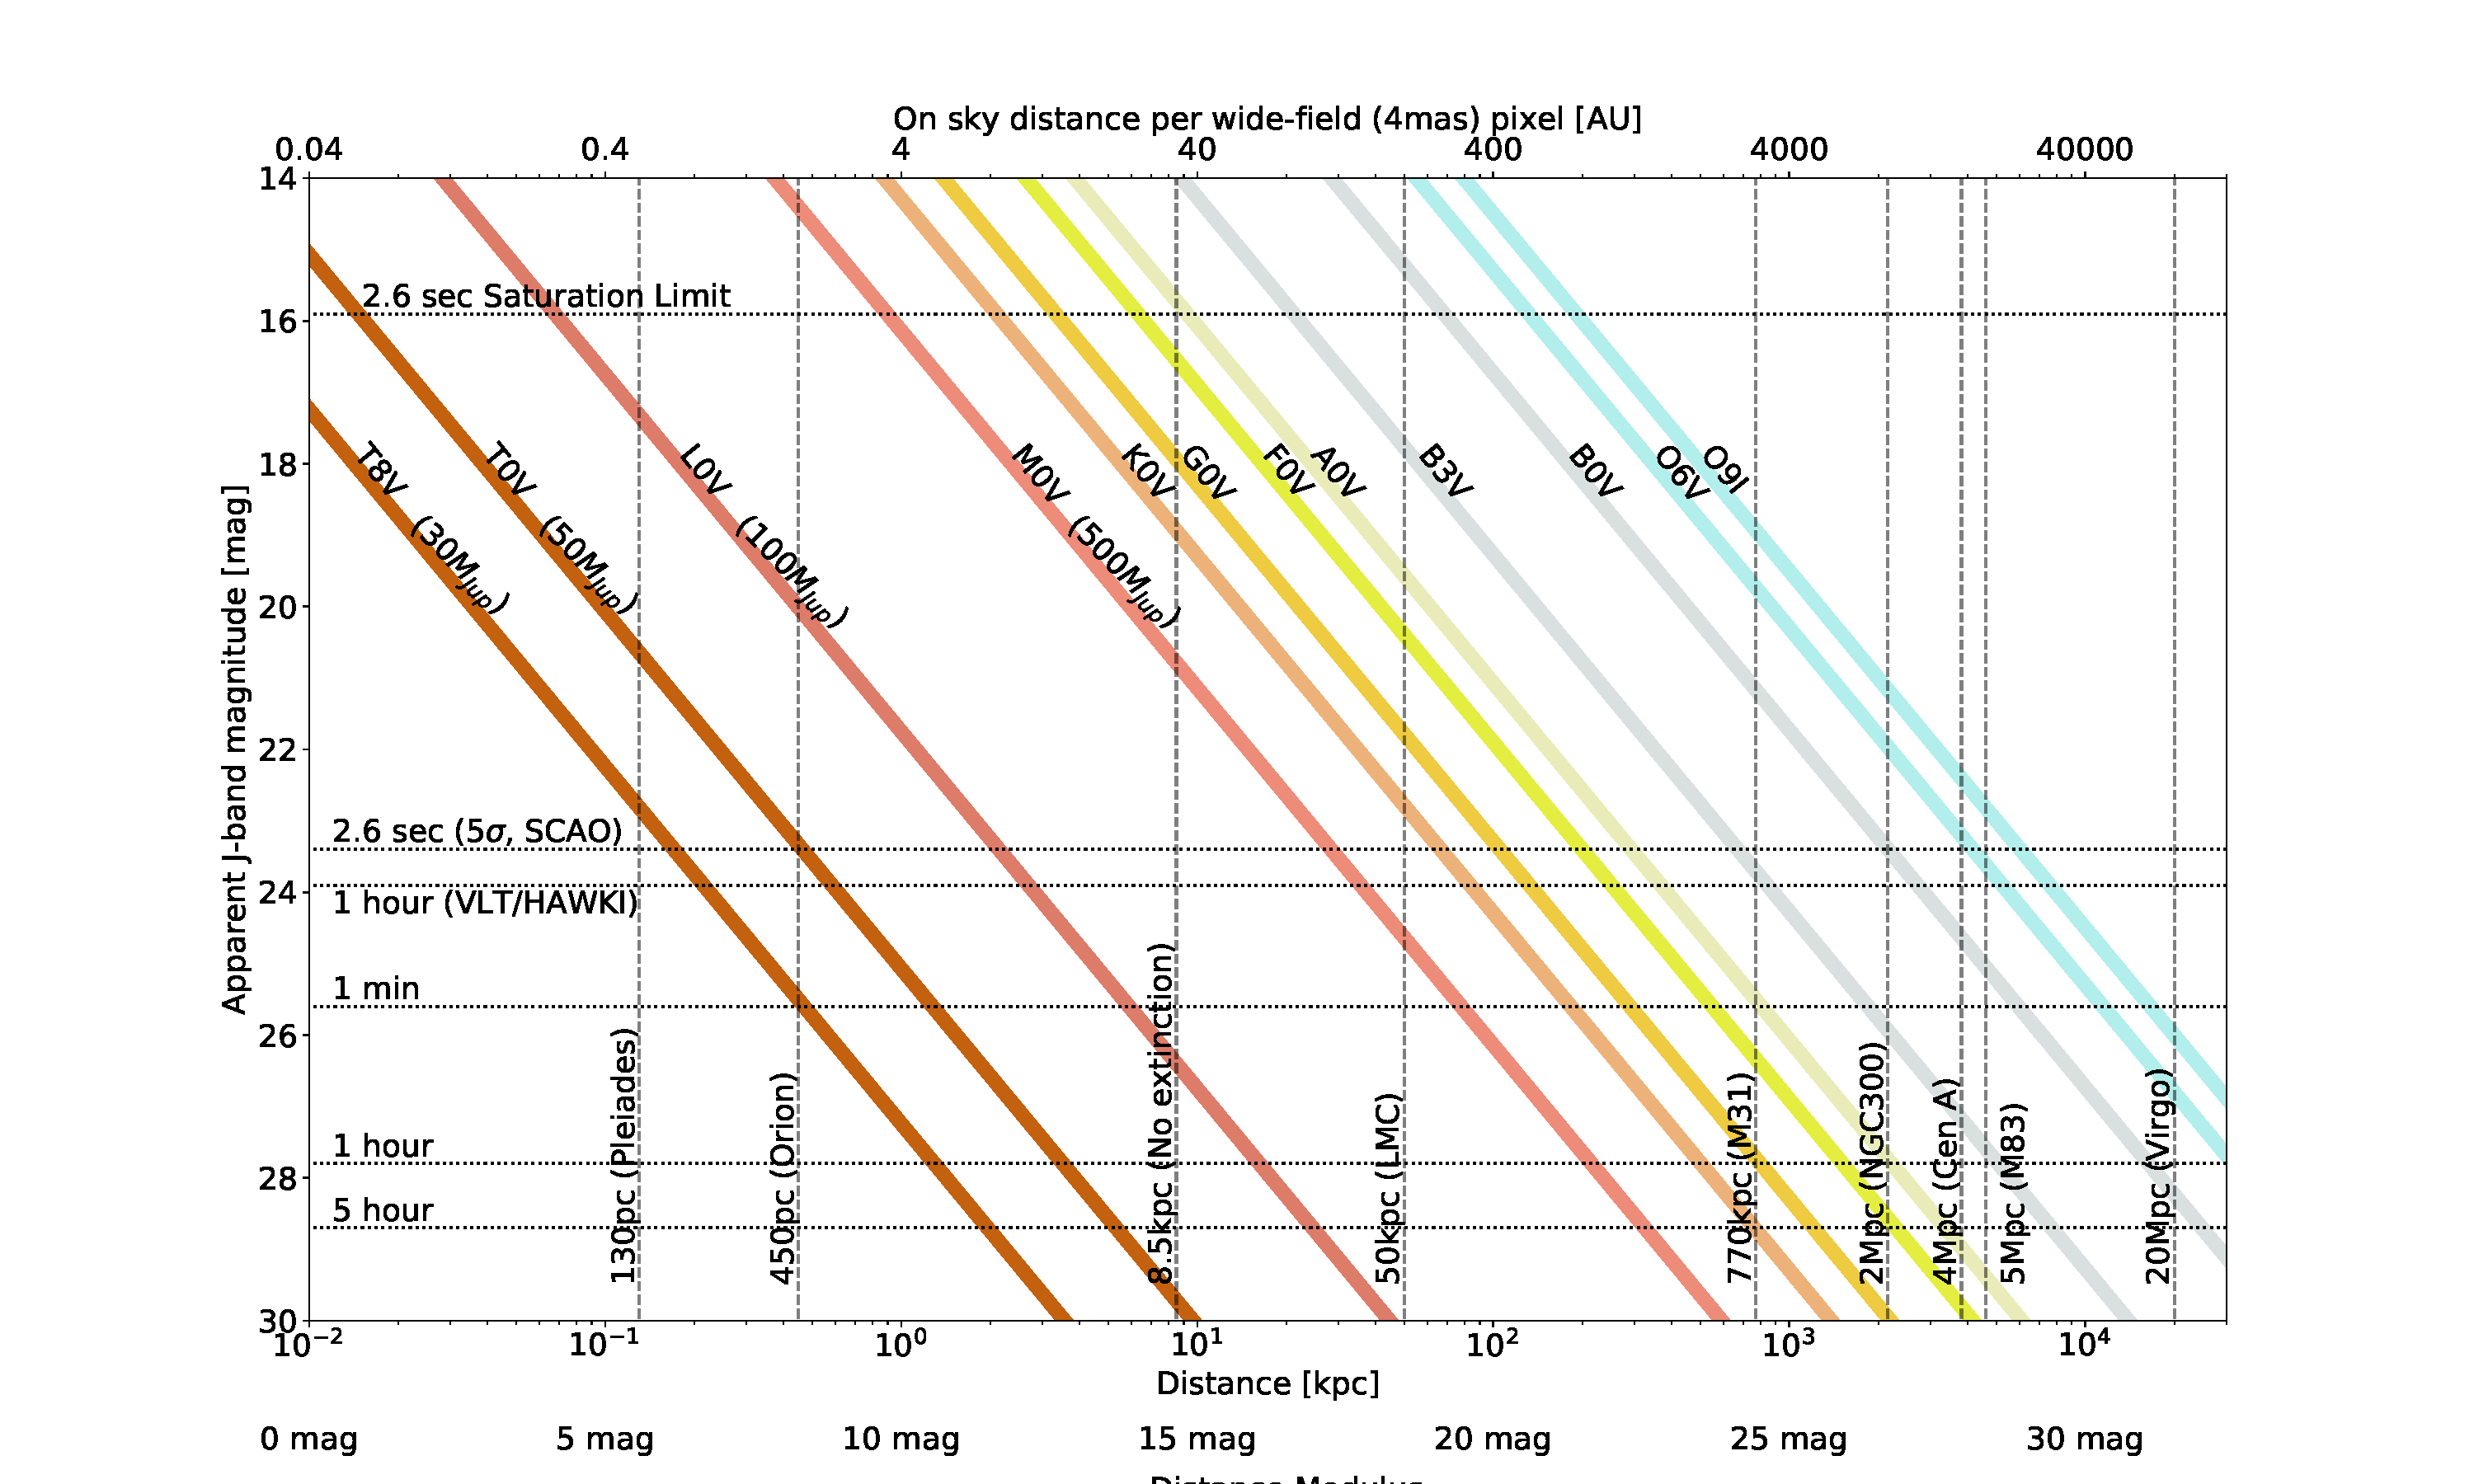
\includegraphics[width=\textwidth]{images/spec_type_vs_dist_J}

    \caption{The coloured lines represent the apparent magnitude of the major spectral types with increasing distance.
    The dashed horizontal lines, unless otherwise stated, represent the $5\sigma$ detection limits for various exposure times with MICADO.
    The intersection of a coloured line with a horizontal dotted line indicates that this type of main-sequence star will no longer be detectable by MICADO at the distance of the position of the intersection on the horizontal axis.
    As a reference, the dashed vertical lines show distances to well known astronomical objects. 
    % It is worth noting that what HAWK-I require 1\,hour to detect, will be detectable by MICADO in a minimum DIT (2.6\,seconds). While this comparison may seem ludicrous, the ELT has a primary mirror $\sim 20\times$ larger that of UT4 at the VLT and the smaller plate scale of MICADO means a factor of $\sim 35\times$ less background flux per pixel.
    }
    
    \label{fig:MS_distances}
    
\end{figure*}


\subsection{Accuracy of the SimCADO sensitivity predictions}
\label{subsec:MICADO_accuracy}

\begin{figure*}
    \centering
    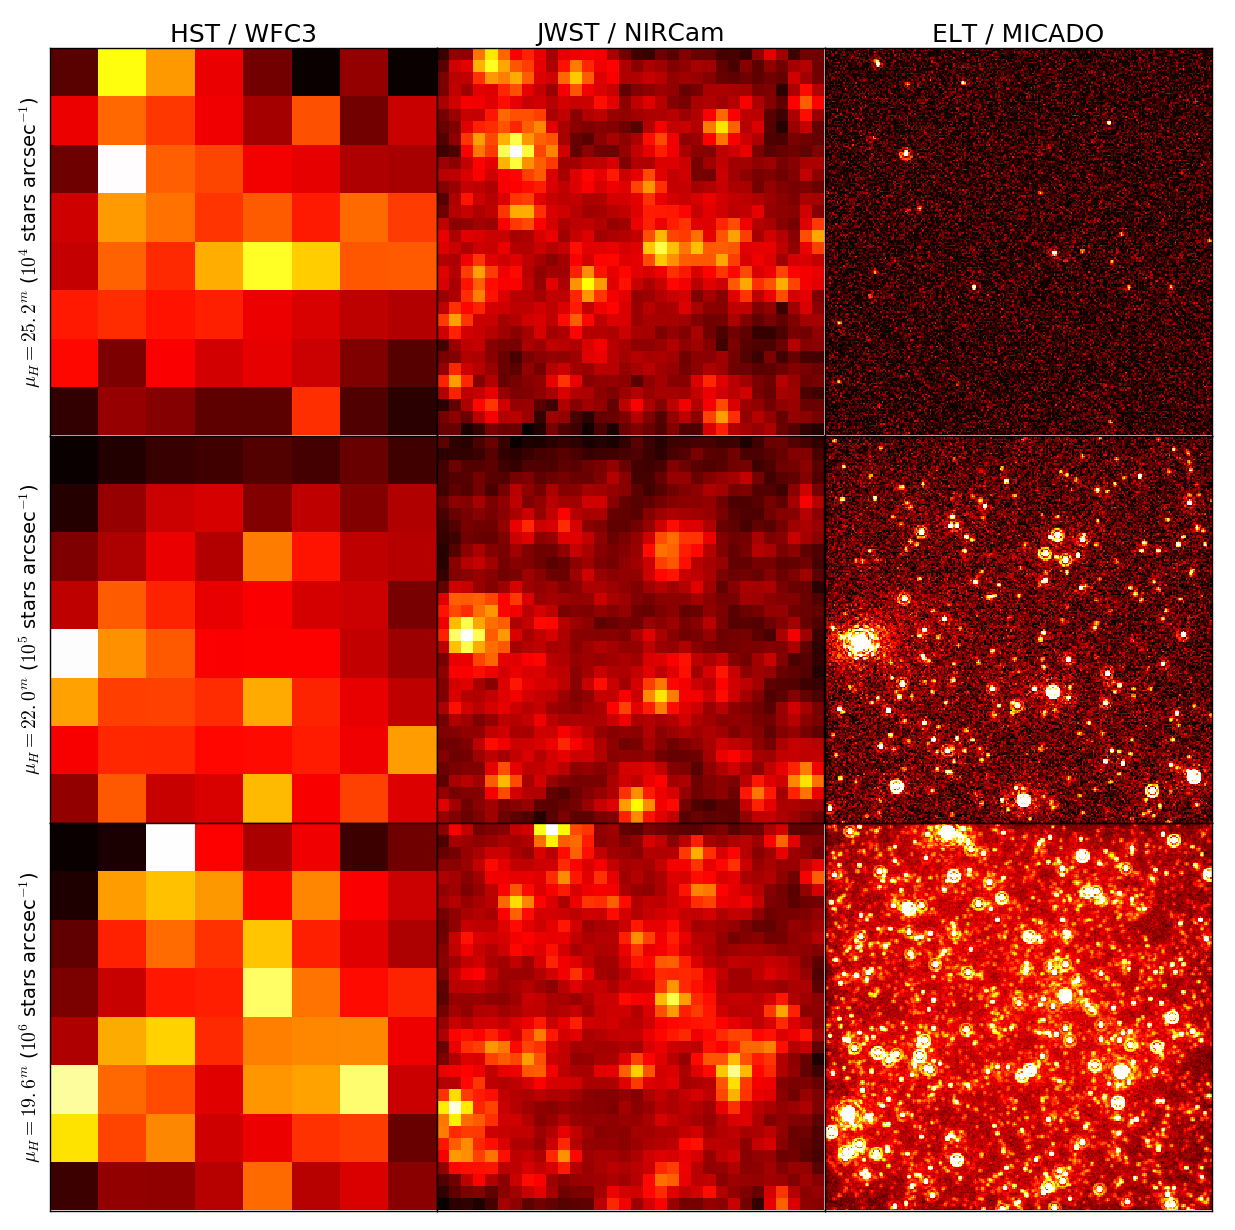
\includegraphics[width=\textwidth]{images/Virgo_old_stellar_pop_HST_JWST_ELT_H_band}
    
    \caption{An illustration of the improvement in resolution that MICADO will provide for observations of densely populated regions compared to HST and JWST.
    The three rows of 1"x1" images show the low (top, $\mu_H=25.2^m$), medium (centre, $\mu_H=22.0^m$) and high (bottom, $\mu_H=19.6^m$) surface brightness regions of an elliptical galaxy at a distance of 18 Mpc - approximately the distance of the Virgo cluster.
    These simulated images were created using configuration files for SimCADO which mimic the optical systems of HST/WFC3, JWST/NIRCam and ELT/MICADO.  
    }
    \label{fig:stellar_field_comp}

\end{figure*}

The accuracy of SimCADO simulations was verified by comparing simulated images with real HAWK-I observations.
Furthermore, estimates from SimCADO images of the detection and saturation limits for observations with MICADO fall within 0.1\m of the values given by the ELT exposure time calculator (after normalising the two optical train configurations).
These two results give us confidence that MICADO's sensitivity can be accurately predicted from simulations with SimCADO.
These simulations have however been conducted using several simplifications.
For example, the atmospheric conditions were assumed to mirror those of the average night at Paranal.
Given that the NIR sky background can vary up to $\sim 0.2$\m within 15\,minutes \citep{moreels08} and that it is also dependent on the level of water in the air as well as the airmass of the pointing, it is clear that the true detection limits of MICADO will vary from this first round of predictions with SimCADO.
Furthermore, the PSF used for the current round of SimCADO predictions was uniform across the field of view.
This will definitely not be the case.
Reductions in the Strehl ratio of $>50\,\%$ over the MICADO field of view are expected for SCAO observations \citep{clenet2015}.
Such variations will have a marked impact on sensitivity in the outer regions of the MICADO focal plane.
Readers interested in simulating observations at large distances (>10 arcsec) from a SCAO NGS are directed to look into the python package AnisoCADO (\url{https://anisocado.readthedocs.io/}) in conjunction with SimCADO.

Another challenge for estimating the performance of the telescope and instrument will be the ELT's PSF.
Accurate photometry of bright sources, extracting faint sources that are covered by the wings of the brighter sources, and accurate astrometry all rely on accurate knowledge of the shape of the PSF.
As can be seen in Fig.~\ref{fig:stellar_field_comp}, the segmented nature of the diffraction spikes of the SCAO PSF could easily confuse a star finding algorithm.
Additionally, the PSF will rotate with respect to the field over the course of an observing run due to the ELT's alt-azimuth mount.
Arguably though, this may prove advantageous as it will provide a natural rotational dithering, which may smooth out the sharp features of the PSF.
An alternative approach would be to deconvolve the images with a spatially varying model of the PSF.
This would however require multiple descriptions of the PSF for each detector frame, which could slowly become a challenging data management task.
Whether this task belongs in the automated data pipeline or is left to the user is still undecided.
A different approach would be to use a blind deconvolution algorithm \citep{vorontsov2017}.
Recent results are encouraging, although it remains to be seen how well this approach works for strong spatial variations in the PSFs.
In any case, the complex PSF of the ELT will present a challenge to standard data analysis techniques.
How the PSF artefacts of bright stars affect the surrounding environment is a question that should be considered in the earliest stages when planning observations with the ELT and MICADO.
